\documentclass[12pt]{article}
\usepackage[paperheight=210mm,paperwidth=148mm,top=2cm,bottom=2cm,left=1cm,right=1cm]{geometry}  % A5 paper
\usepackage{background}
\backgroundsetup{
    scale=1,
    opacity=0.1,
    angle=0,
    color=black,
    contents={%
        
\includegraphics[width=\paperwidth]{background}
    }
}
%%%%%%%%%%%%%%%%%%%%%%%%%%%%%%%%%%%%%%%%
\usepackage[utf8]{inputenc}
\usepackage[brazil]{babel}
\usepackage{titlesec}
%\usepackage[all]{hypcap}
\usepackage{multirow}
%\usepackage{tikz}
\usepackage{ctable}
%%%%%%%%%%%%%%%%%%%%%%%%%%%%%%%%%%%%%%%%
\renewcommand{\familydefault}{\sfdefault}
% \titleformat{\chapter}[display]
% {\bfseries\LARGE\sffamily}{\chaptertitlename}{10pt}{\LARGE}
% \titlespacing*{\chapter}{0pt}{10pt}{10pt}
% \numberwithin{table}{chapter}


\begin{document}
% Cover
\newgeometry{left=0cm, bottom=0cm, top=0cm, right=0cm}
\thispagestyle{empty}
\noindent  % To remove the unwanted white space.

\includegraphics{capa}
\NoBgThispage

\clearpage

\restoregeometry

\newpage

Olá,

no dia 16 de Maio de 2016 realizou-se o pré-evento para o SciPy Latin America
2016 no Centro de Informática e Automação do Estado de Santa Catarina S.A..
Foram mais de 6 horas de atividades nas quais os 13 participantes aprenderam um
pouco de Python, Git e LaTeX.
Agradecemos a ajuda de todos que estiveram envolvidos na realização do evento.

Att, \\
\indent Ivan Ogasawara \\
\indent Presidente da SciPy Latin America 2016


\newpage

\section*{Programa}

O programa divulgado para os participantes foi

% TODO Adicionar link para slides ou apresentação.
\begin{tabular}{cp{0.4\textwidth}l}
  \textbf{Horário} & \textbf{Título} & \textbf{Instrutor} \\
  9h-10h & SciTools Install Fest: Python - Anaconda, LaTeX, Git & \\
  10h10-12h10 & Introdução ao Python & Mário Sergio \\
  12h10-13h40 & Almoço \\
  13h40-14h40 & LaTeX - Automatizando a criação de PDFs com LaTeX+Python & Melissa Mendonça \\
  14h50-15h50 & Git/GitHub & Matheus Magrin \\
  16h00-17h00 & Open Science / Ciência Aberta & Ivan Ogassavara \\
\end{tabular}

\begin{figure}[!htb]
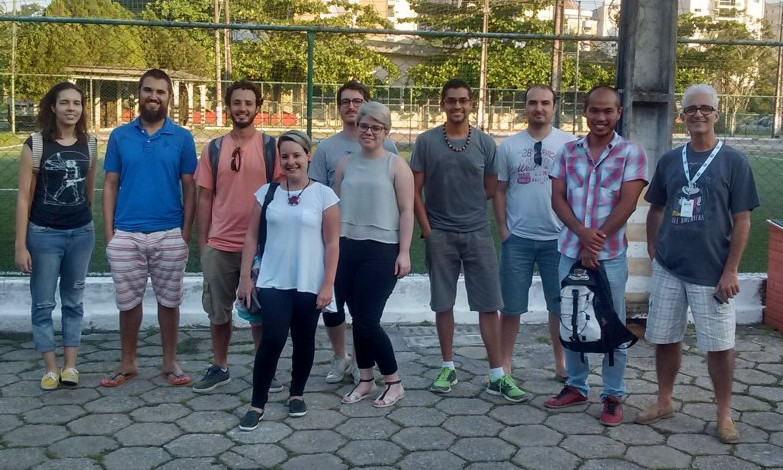
\includegraphics[width=\textwidth]{../../media/photos/pre4-cut}
\caption{Instrutores}
\end{figure}

Esse cronograma foi parcialmente cumprido. O horário da última atividade foi cedido para que o tema
de Git fosse visto com mais aprofundamento. Mesmo com essa extensão, não foi possível passar todo o
conteúdo programado. Foi levantada a opção de concluir essa palestra em outro dia.

No período da manhã as atividades ocorreram dentro do horário previsto, porém muitos dos participantes
não chegaram no horário agendado. Como este período estava destinado à instalação de softwares e também
seria um espaço para as pessoas poderem se conhecerem e conversarem, a primeira atividade ocorreu bem.

% TODO Descrever duração das atividades.
Duração das atividades realizadas:

\begin{tabular}{cp{0.4\textwidth}l}
  \textbf{Horário} & \textbf{Título} & \textbf{Instrutor} \\
  9h-10h & SciTools Install Fest: Python - Anaconda, LaTeX, Git & \\
  10h10-12h10 & Introdução ao Python & Mário Sergio \\
  12h10-13h40 & Almoço \\
  13h50-14h50 & LaTeX - Automatizando a criação de PDFs com LaTeX+Python & Melissa Mendonça \\
  15h00-17h00 & Git/GitHub & Matheus Magrin \\
\end{tabular}

A programação inicial prevista não levava em consideração a complexidade dos sistemas de versionamento e
do Git. Deveria ter sido deixado um período de ao menos 2 horas para esta atividade.

% TODO Descrever interrupções.
Durante o transcorrer das atividades não houve interrupções.

% TODO Descrever variação no público. Eg pessoas que só apareceram na manha ou
Do período da manhã apenas 3 pessoas não continuaram as atividades da tarde.
% só a tarde.
Durante o período da tarde recebemos mais 3 pessoas.

\newpage

\section*{Público}

Entre os dias 8 de Abril e 16 de Abril (quando o evento foi realizado)
tivemos 29 inscritos (26 homens e 3 mulheres) dos quais apenas 13 apareceram no
dia (8 homens e 5 mulheres).

\begin{figure}[!htb]
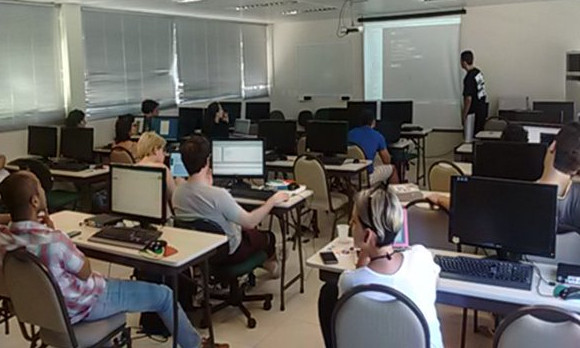
\includegraphics[width=\textwidth]{../../media/photos/pre0-cut}
\caption{Instrutores}
\end{figure}

Esperávamos em torno de 50\% de presença tendo em vista que não cobramos
inscrição dos participantes.
Algumas pessoas que não tinham feito inscrição antecipada apareceram e puderam
participar do evento.

% TODO Adicionar sugestões para aumentar o número de presentes.
A divulgação do evento foi realizada durante apenas uma semana, que pode ter resultado em um número
baixo de inscritos. Outro fator encontrado é que neste dia foi realizado a prova de proficiência de
TOEFL na UFSC e muitos interessados não puderam ir pois iriam participar deste exame.
\newpage

\section*{Repercussão}

Infelizmente nossa equipe só publicou 4 tweets durante o evento que foram
apreciadas ou repetidas por algumas poucas pessoas.
A pessoa a cargo da cobertura do evento nas redes sociais era novato nessa área
e acabou publicando os tweets na conta pessoal e não na conta do SciPy Latin
America de forma que os tweets não foram publicadas na página da comunidade no
Facebook.

Alguns dos participantes manifestaram interesse em montar um grupo de estudo de Python. O Ivan
Ogasawara já está cuidando de um grupo de estudo na Universidade Federal de Santa Catarina e
convidou os interessados à participarem do grupo.

Após a realização do evento, foi enviado aos participantes um questionário para recebermos suas
opiniões sobre as palestras e o evento. Foram adicionados ao questionário um levantamento das
pessoas interessadas em assistir a conclusão do tema de git e assistir a palestra sobre ciência
aberta.

Na figura \ref{fig:evento} pode-se ver que o evento, de uma maneira geral, foi satisfatório para
todos os participantes. Nas figuras \ref{fig:python1} a \ref{fig:git3} pode-se ver os gráficos
mostrando as respostas às perguntas sobre as palestras de Python, \LaTeX e Git. As respostas
foram em sua grande maioria positivas (\textit{Regular}, \textit{Bom} e \textit{Muito bom}).

\begin{figure}[p]
    \centering
    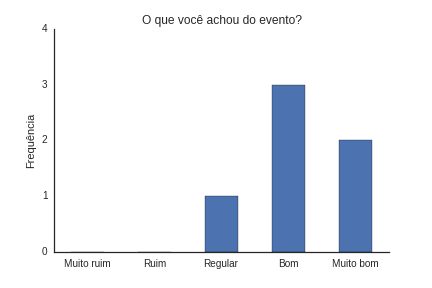
\includegraphics[scale=0.6]{images/evento1.png}
    \caption{\label{fig:evento}O que achou do evento?}
\end{figure}

% Python plots
\begin{figure}[p]
    \centering
    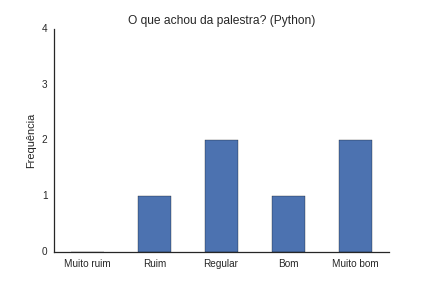
\includegraphics[scale=0.6]{images/python1.png}
    \caption{\label{fig:python1}O que achou da palestra? (Python)}
\end{figure}

\begin{figure}[p]
    \centering
    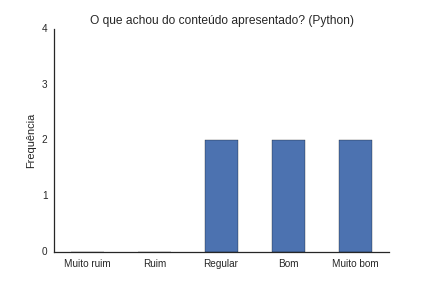
\includegraphics[scale=0.6]{images/python2.png}
    \caption{\label{fig:python2}O que achou do conteúdo apresentado? (Python)}
\end{figure}

\begin{figure}[p]
    \centering
    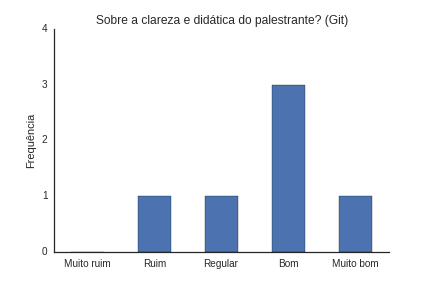
\includegraphics[scale=0.6]{images/python3.png}
    \caption{\label{fig:python3}Sobre a clareza e didática do palestrante? (Python)}
\end{figure}


% LaTeX plots
\begin{figure}[p]
    \centering
    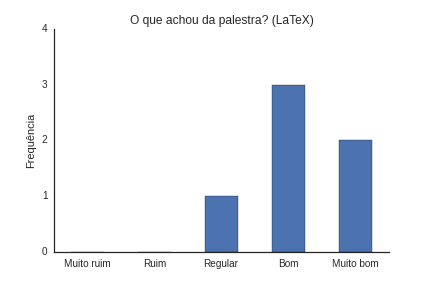
\includegraphics[scale=0.6]{images/latex1.png}
    \caption{\label{fig:latex1}O que achou da palestra? (LaTex)}
\end{figure}

\begin{figure}[p]
    \centering
    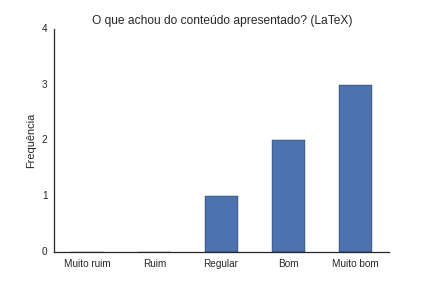
\includegraphics[scale=0.6]{images/latex2.png}
    \caption{\label{fig:latex2}O que achou do conteúdo apresentado? (LaTeX)}
\end{figure}

\begin{figure}[p]
    \centering
    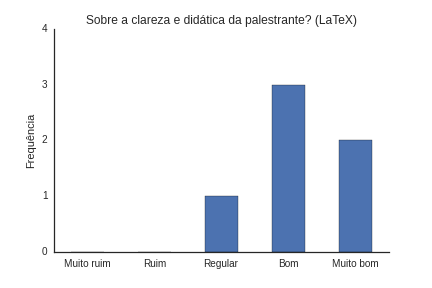
\includegraphics[scale=0.6]{images/latex3.png}
    \caption{\label{fig:latex3}Sobre a clareza e didática da palestrante? (LaTeX)}
\end{figure}


% Git plots
\begin{figure}[p]
    \centering
    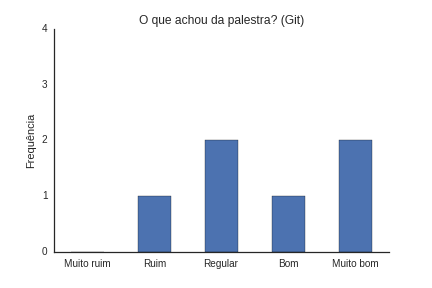
\includegraphics[scale=0.6]{images/git1.png}
    \caption{\label{fig:git1}O que achou da palestra? (Git)}
\end{figure}

\begin{figure}[p]
    \centering
    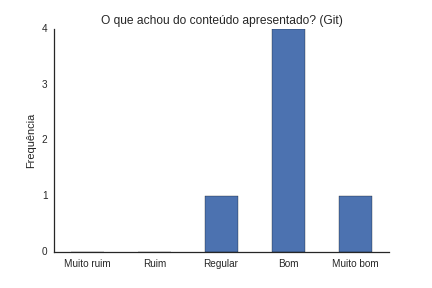
\includegraphics[scale=0.6]{images/git2.png}
    \caption{\label{fig:git2}O que achou do conteúdo apresentado? (Git)}
\end{figure}

\begin{figure}[p]
    \centering
    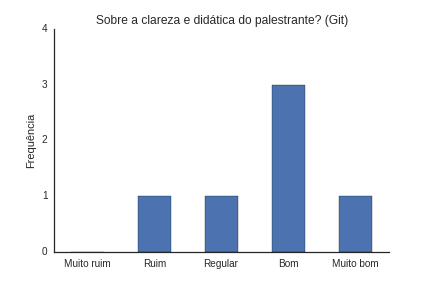
\includegraphics[scale=0.6]{images/git3.png}
    \caption{\label{fig:git3}Sobre a clareza e didática do palestrante? (Git)}
\end{figure}

\newpage

\section*{Finanças}

As despesas para o evento foram

% TODO Adicionar todos os gastos da organização
% incluindo passagens de ônibus e ou gasolina.
\begin{tabular}{p{0.6\textwidth}r}
  \textbf{Descrição} & \textbf{Subtotal} (em R\$) \\
  Locação do espaço & 0,00 \\
  Transporte & 20,00 \\ % TODO Adicionar taxi ou uber. Valor estimado (carro+bus+bicicleta)
  Almoço & 40,00 \\ % TODO Adicionar almoço. Valor estimado (20x4)
  Happy-hour & 0,00 \\ % TODO Adicionar cerveja e lanche
\end{tabular}

% agradecimento

Agradecemos ao Centro de Informática e Automação do Estado de Santa Catarina
S.A. por patrocinar o evento, disponibilizando a infraestrutura utilizada.

Agradecemos também aos palestrantes pelos trabalhos apresentados e a presença da comunidade representada pelos presentes.

% A receita com o evento foi
%
% % TODO Adicionar todos os gastos como doação.
% \begin{tabular}{p{0.6\textwidth}r}
%   \textbf{Descrição} & \textbf{Subtotal} (em R\$) \\
%   Doação anônima & 0,00 \\
% \end{tabular}

\end{document}
